	\section{Circuito RLC diferente (Caso 3)}

\subsection{Parámetros y método}
El circuito analizado es una red RLC serie excitada por una fuente AC de 1 V. La salida se mide en $OUT$, sobre la resistencia $R_1$. Aunque el netlist denomina al circuito ``pasa-altas'', la salida sobre la resistencia presenta una respuesta resonante de banda: disminuye tanto en el extremo bajo como en el alto del barrido.

\begin{table}[H]
\centering
\begin{tabular}{ll}
\toprule
Parámetro & Valor \\
\midrule
Frecuencia de inicio y final & 10 Hz y 100 kHz \\
Tipo de barrido & Lineal, 400 puntos \\
Fuente $V_1$ & 1 V AC, $0^\circ$ \\
$C_1$ & 1 $\mu$F \\
$L_1$ & 10 mH \\
$R_1$ & 1 k$\Omega$ \\
Salida & $V(OUT)$ sobre $R_1$ \\
Formulación & Tableau completa \\
\bottomrule
\end{tabular}
\caption{Parámetros del circuito RLC diferente.}
\end{table}

\begin{figure}[H]
\centering
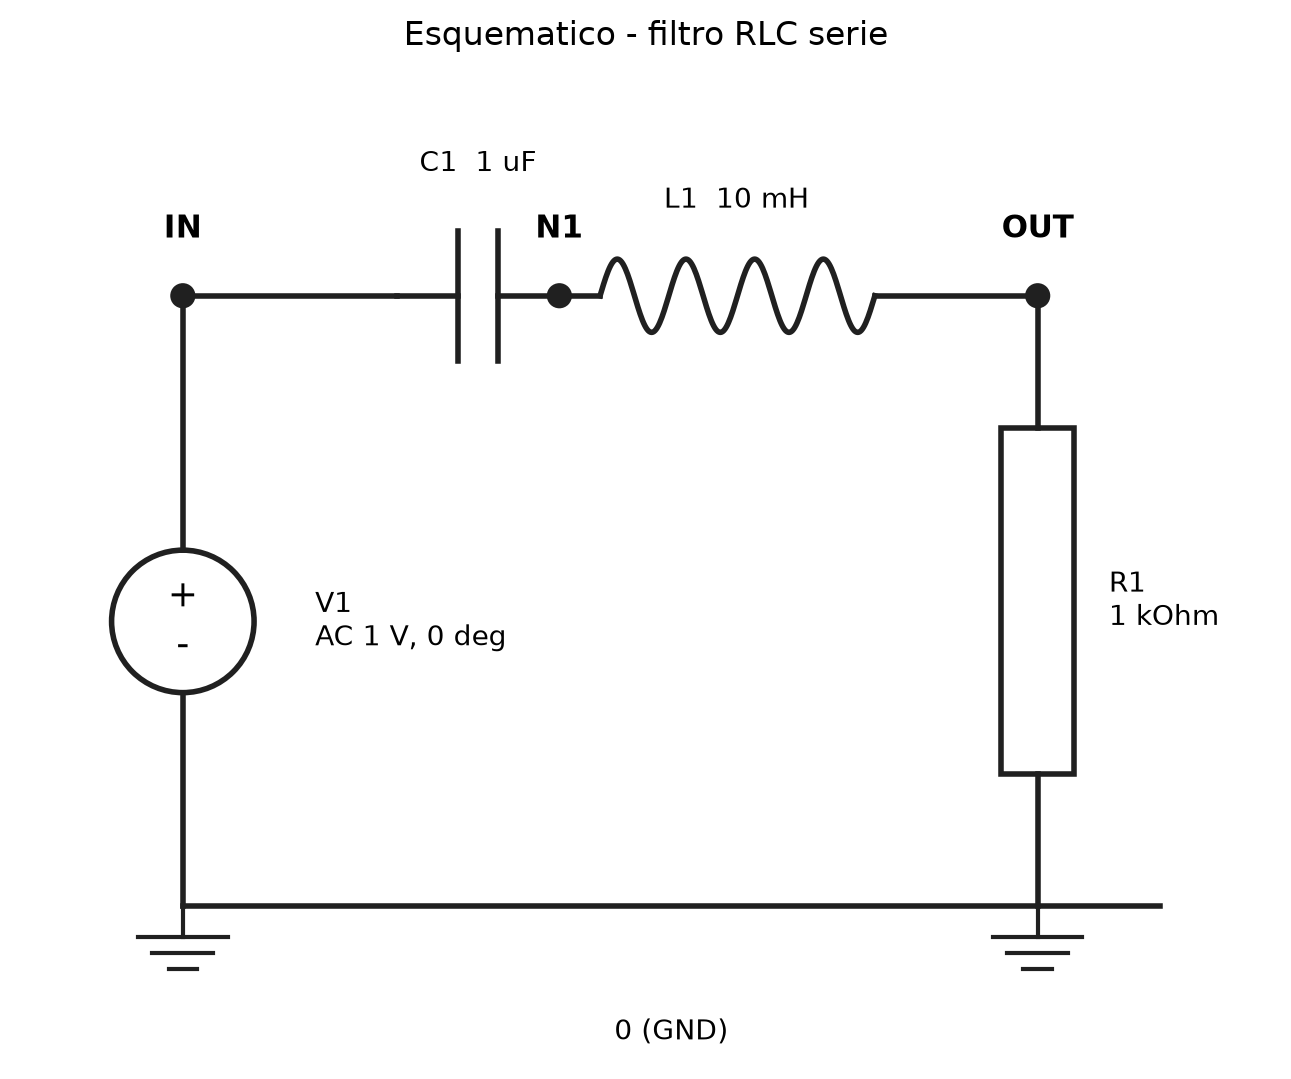
\includegraphics[width=0.78\linewidth]{3_circuito_dif_agent/plots/esquematico_filtro_pasa_altas.png}
\caption{Esquemático del circuito RLC serie.}
\end{figure}

\subsection{Topología, Tableau y validación}
La validación del netlist fue \textbf{Satisfactorio}. El circuito se ensambló mediante Tableau completo, de dimensión $11\times11$. La validación del sistema Tableau a 10 Hz fue \textbf{Satisfactorio} en sus cinco comprobaciones; el número de condición reportado fue $3.4574\times10^6$. En el barrido AC, el estado global fue \textbf{Satisfactorio} y los 400 puntos se validaron.

\begin{figure}[H]
\centering
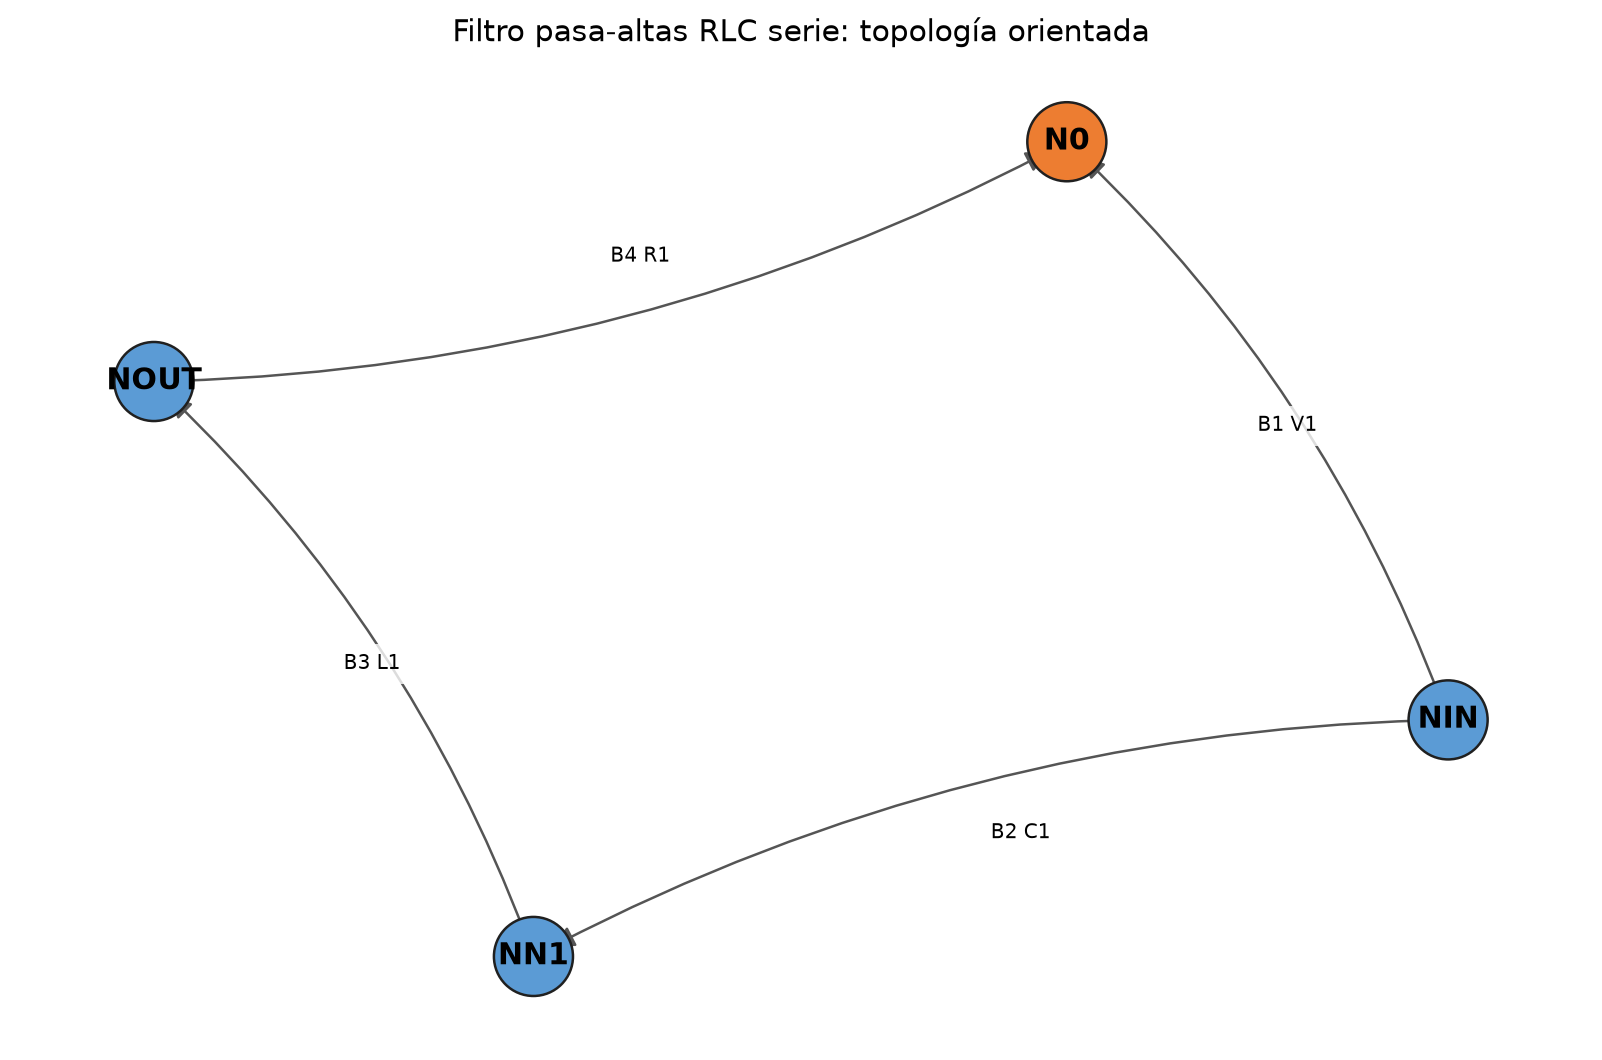
\includegraphics[width=0.78\linewidth]{3_circuito_dif_agent/plots/graph.png}
\caption{Grafo orientado de la red RLC.}
\end{figure}

\begin{figure}[H]
\centering
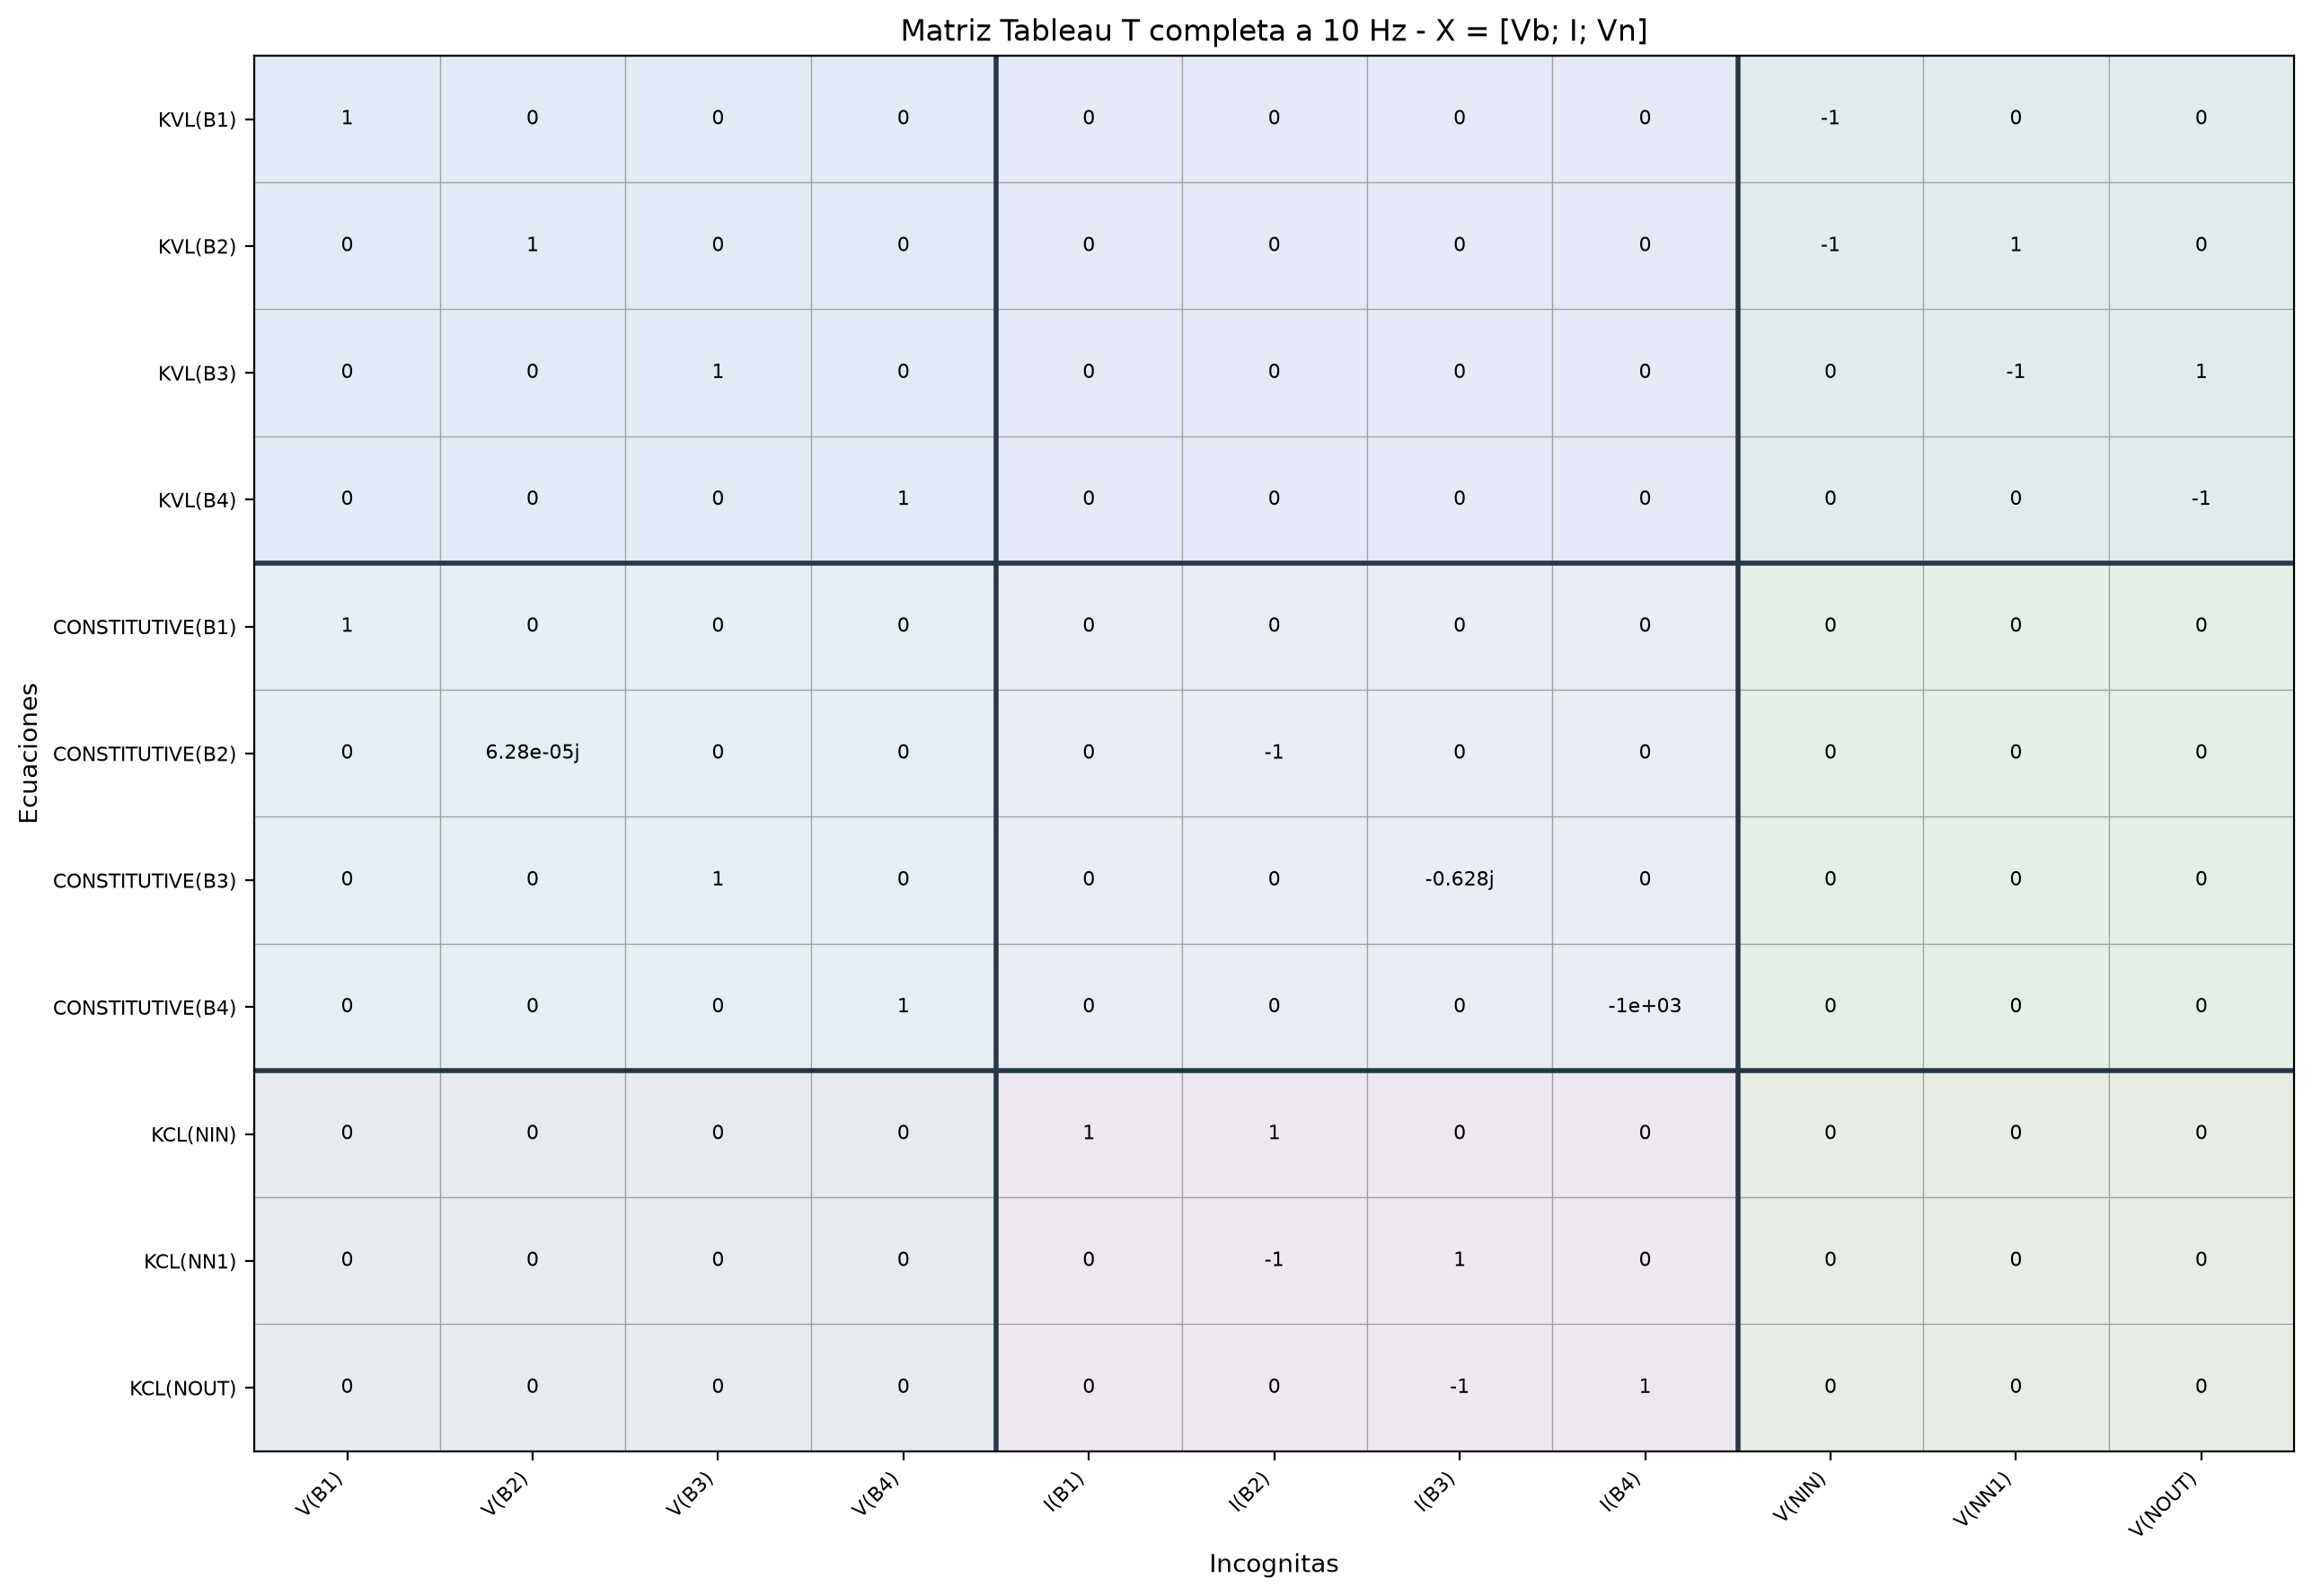
\includegraphics[width=0.95\linewidth]{3_circuito_dif_agent/plots/tableau_T_10Hz.png}
\caption{Matriz Tableau completa $T$ a 10 Hz, con $X=[V_b; I; V_n]$.}
\end{figure}

\subsection{Resultados del analisis en AC del Agente y HSPICE}
El observable es $V(OUT)/V(IN)$. Como la fuente AC tiene amplitud de 1 V, la magnitud de la transferencia coincide numéricamente con la magnitud del voltaje de salida en voltios. Los valores siguientes proceden del Agente y corresponden al inicio, al máximo muestreado del barrido y al final.

\begin{table}[H]
\centering
\begin{tabular}{lrrr}
\toprule
Punto & Frecuencia (Hz) & Magnitud (dB) & Fase ($^\circ$) \\
\midrule
Inicio & 10 & -24.0532 & 86.4046 \\
Máximo muestreado & 1513.6090 & -0.0004383 & 0.5756 \\
Fin & 100000 & -16.0701 & -80.9547 \\
\bottomrule
\end{tabular}
\caption{Valores representativos de $V(OUT)/V(IN)$ obtenidos con Tableau.}
\end{table}

En esos mismos puntos, la magnitud de $V(OUT)$ reportada por el Agente fue 0.0627107 V, 0.9999495 V y 0.1572156 V, respectivamente.

\begin{figure}[H]
\centering
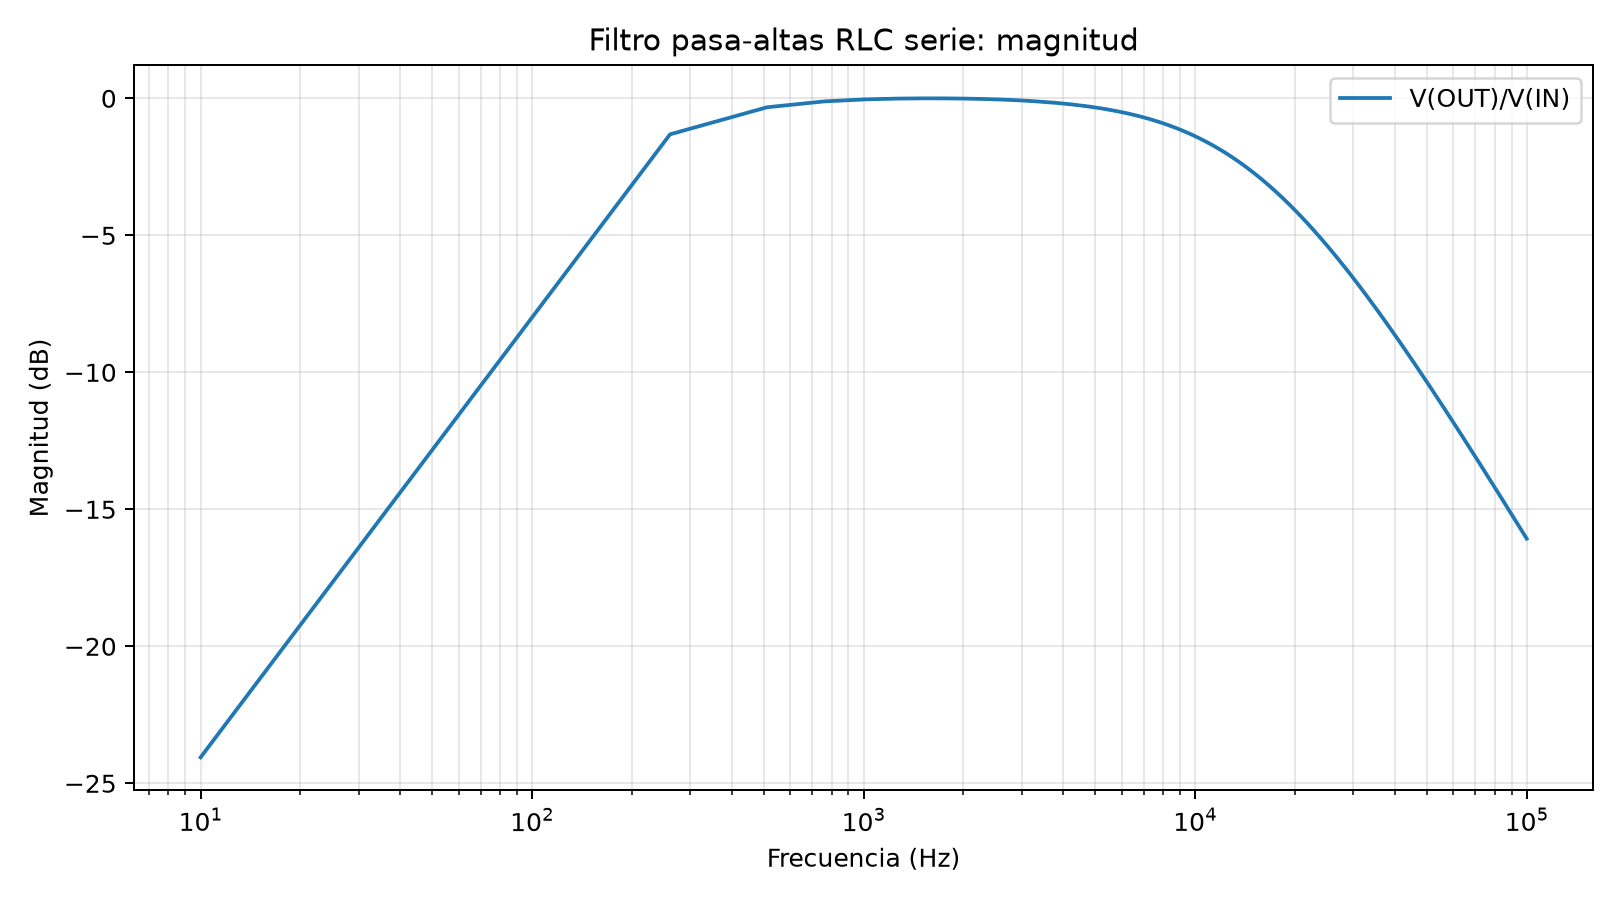
\includegraphics[width=0.70\linewidth]{3_circuito_dif_agent/plots/magnitude.png}
\caption{Gráfica de Magnitud en dB de la función de transferencia $H(w)$ obtenida por el agente.}
\end{figure}


\begin{figure}[H]
\centering
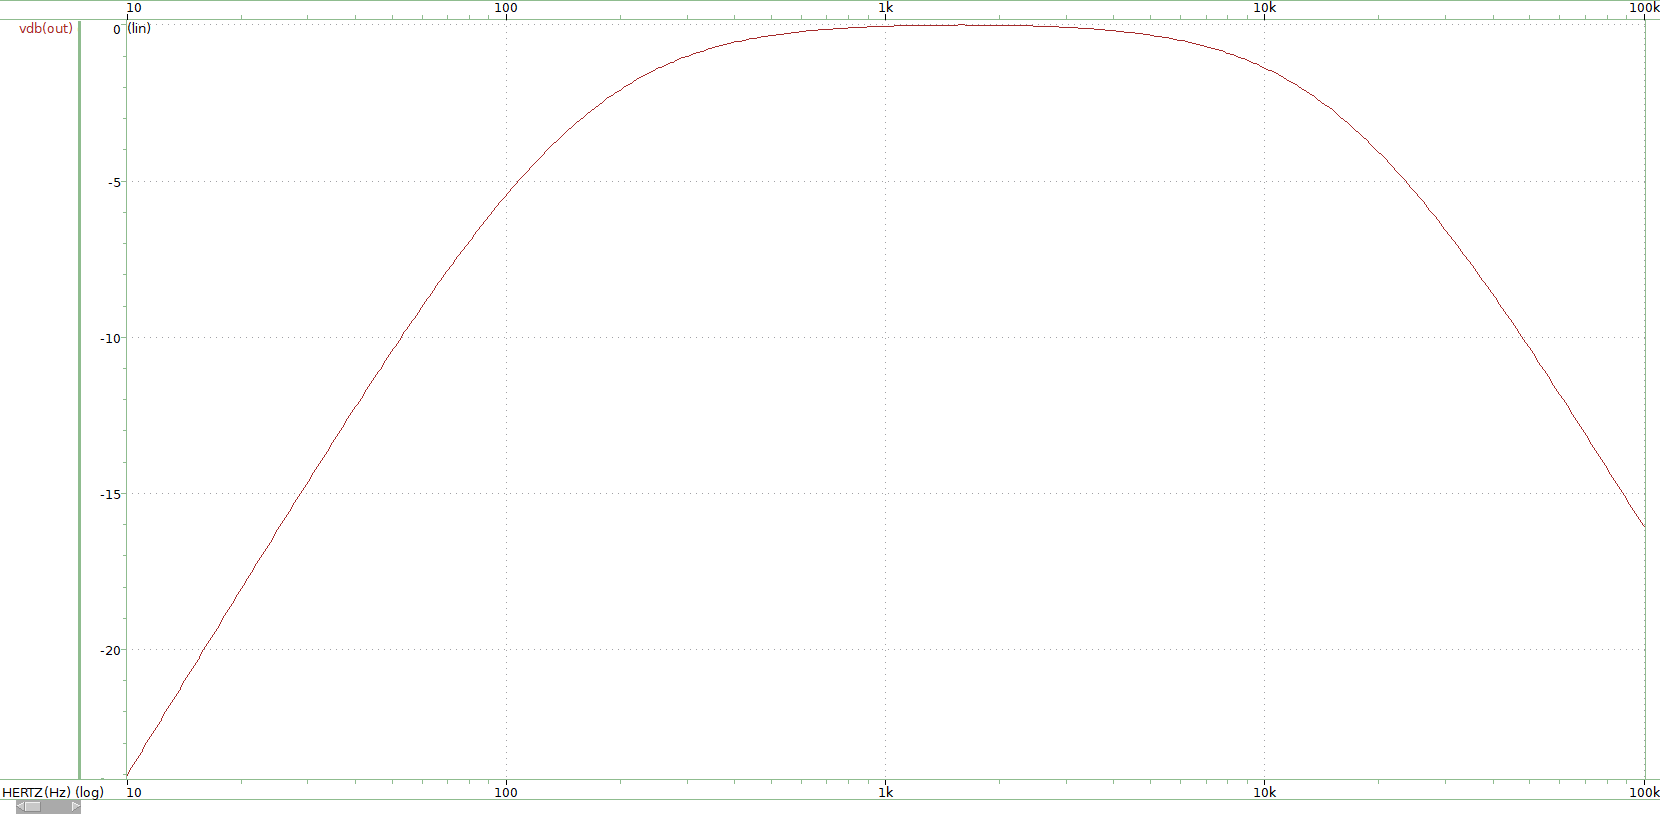
\includegraphics[width=0.70\linewidth]{3_circuito_dif_HSPICE/magnitude_db.png}
\caption{Gráfica de Magnitud en dB de la función de transferencia $H(w)$ obtenida por HSPICE.}
\end{figure}

\begin{figure}[H]
\centering
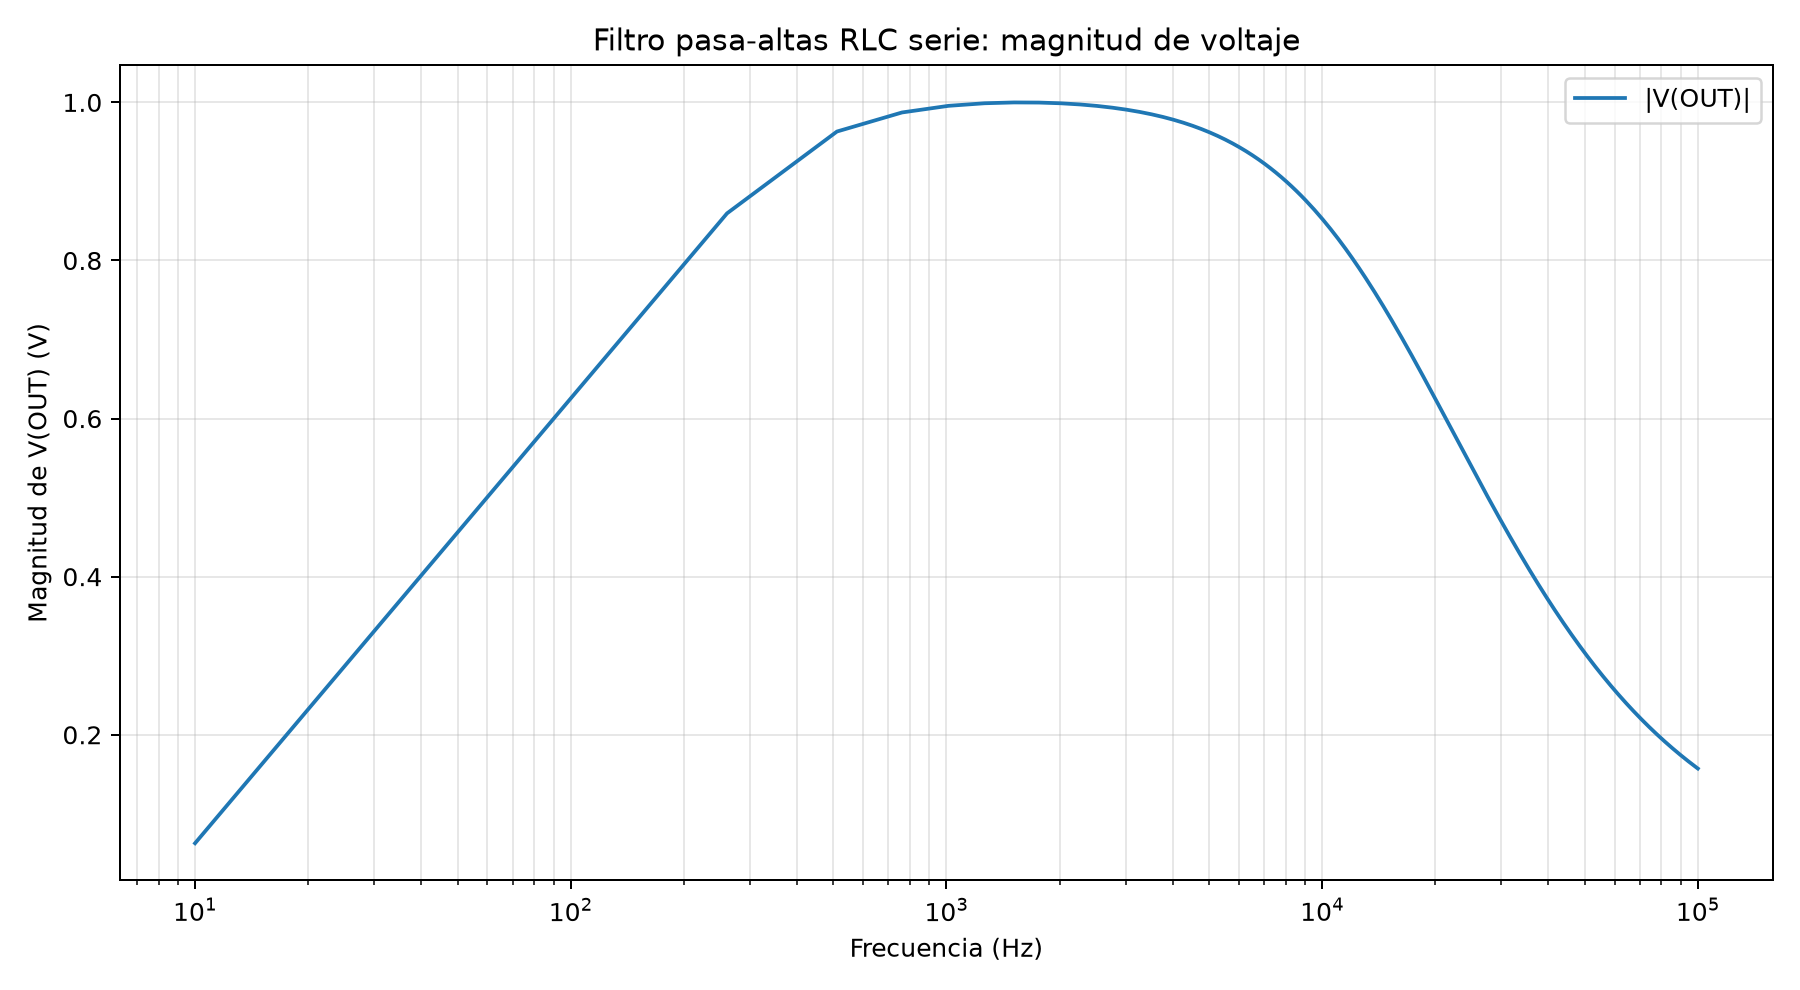
\includegraphics[width=0.70\linewidth]{3_circuito_dif_agent/plots/magnitude_voltage.png}
\caption{Gráfica de Magnitud en Voltaje de $V\_OUT$ obtenida por el agente.}
\end{figure}

\begin{figure}[H]
\centering
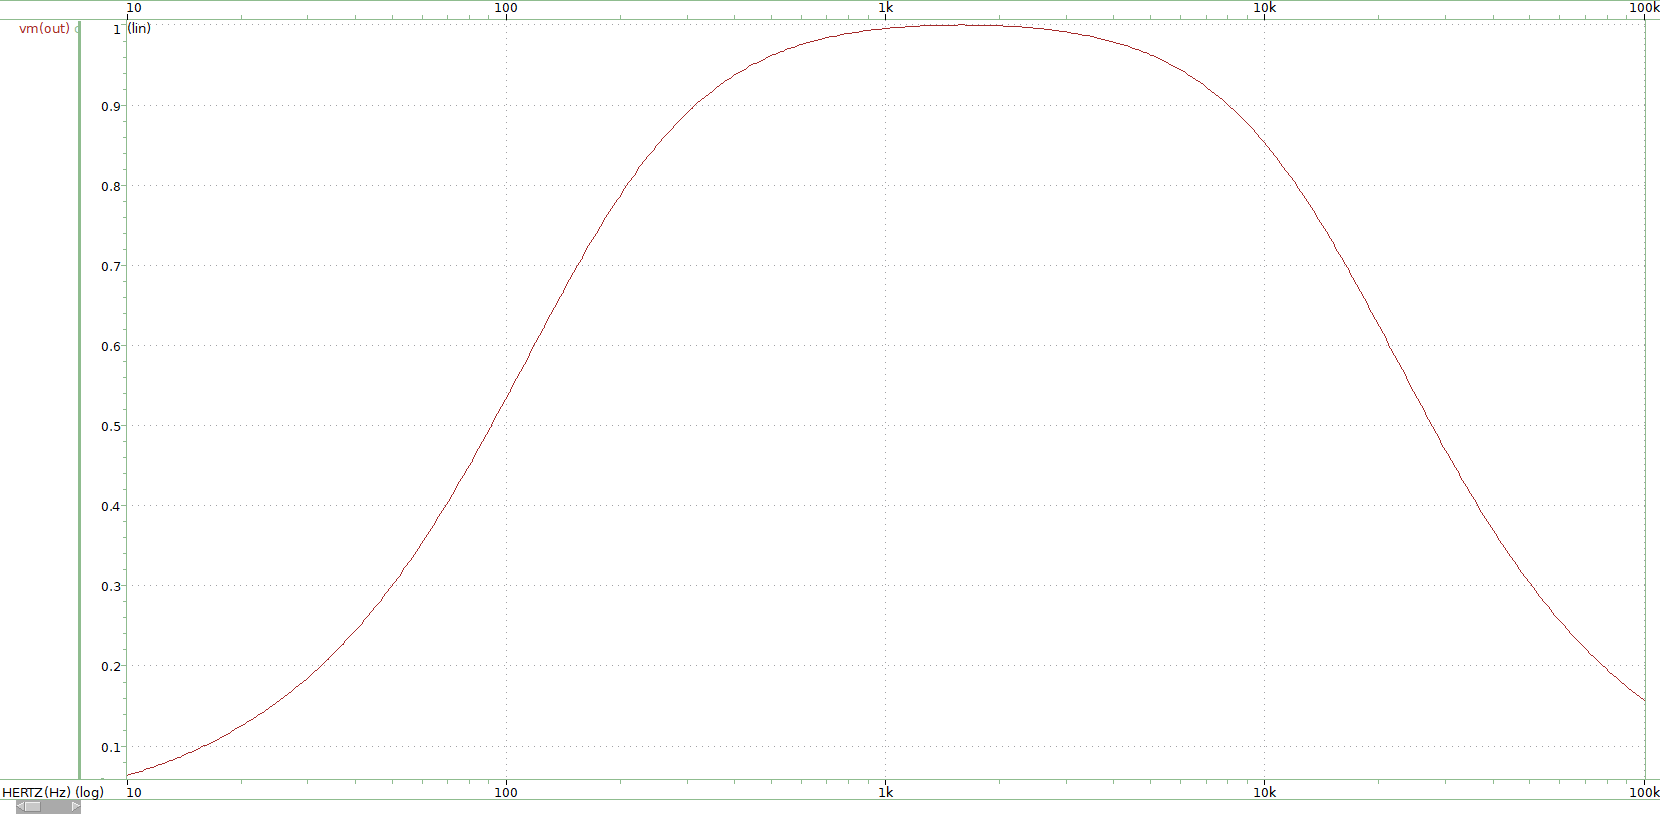
\includegraphics[width=0.70\linewidth]{3_circuito_dif_HSPICE/magnitude_voltage.png}
\caption{Gráfica de Magnitud en Voltaje de $V\_OUT$ obtenida por HSPICE.}
\end{figure}

\begin{figure}[H]
\centering
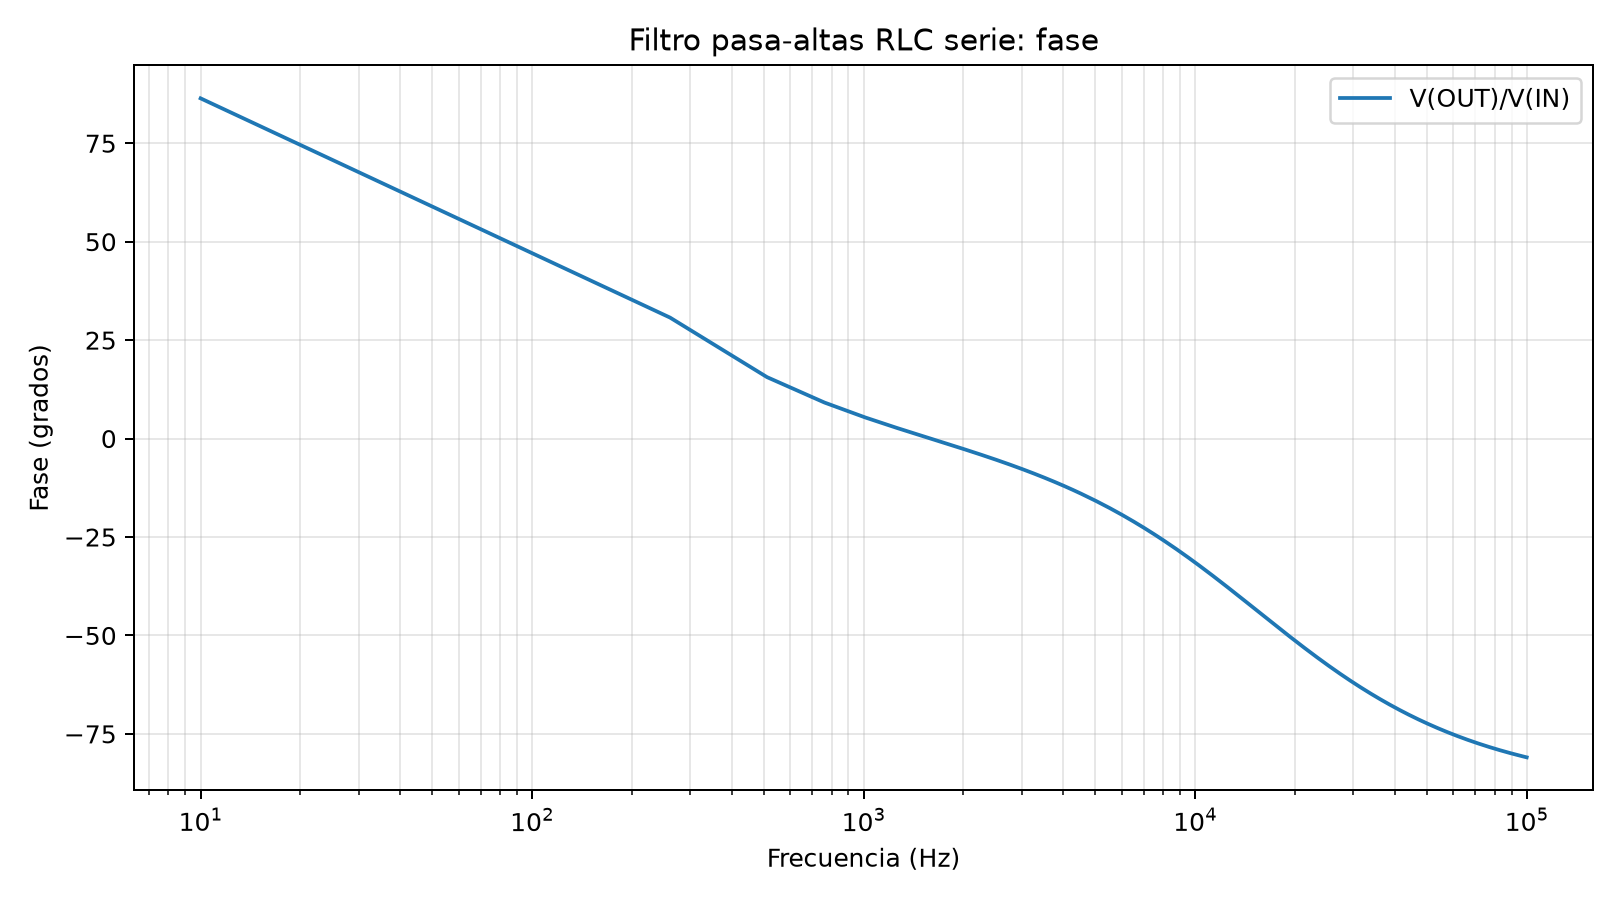
\includegraphics[width=0.70\linewidth]{3_circuito_dif_agent/plots/phase.png}
\caption{Gráfica de Fase de la función de transferencia $H(w)$ obtenida por el agente.}
\end{figure}

\begin{figure}[H]
\centering
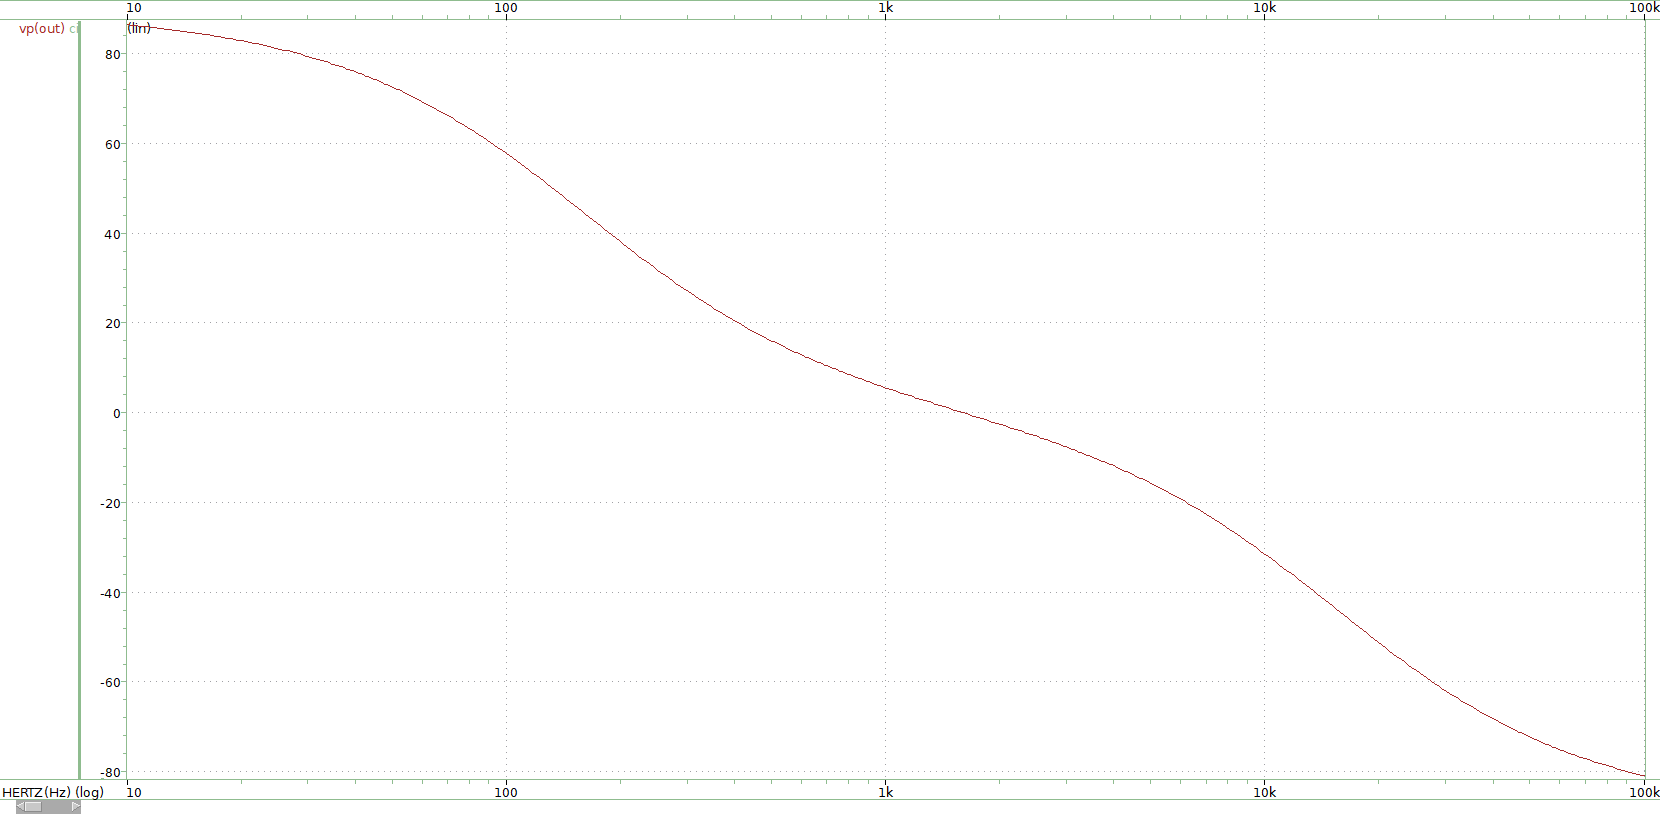
\includegraphics[width=0.70\linewidth]{3_circuito_dif_HSPICE/phase.png}
\caption{Gráfica de Fase de la función de transferencia $H(w)$ obtenida por HSPICE.}
\end{figure}


\subsection{Comparación con HSPICE}
La referencia corresponde a los datos obtenidos por HSPICE usando un circuito RLC, con fuente de entrada de 1 V y barrido DEC de 401 puntos. El agente utilizó un barrido LIN de 400 puntos. Se compararon solo las frecuencias coincidentes exactas de 10 Hz y 100 kHz, sin interpolar ni alterar unidades. En ambas simulaciones, debido a que $V(IN)=1$ V, el voltaje de salida es numéricamente igual a $H(w)=V(OUT)/V(IN)$.

La herramienta \texttt{compare\_reference.py} comparó los fasores complejos de la transferencia, con tolerancias absoluta $10^{-6}$ y relativa $2\times10^{-5}$. Los fasores, errores y estados se transcriben de su artefacto de salida.

\begin{table}[H]
\centering
\small
\begin{tabularx}{\linewidth}{lXX}
\toprule
Frecuencia & Agente $H(w)$ & HSPICE: $H(w)$ \\
\midrule
10 Hz & $3.93262687\times10^{-3}+j6.25872297\times10^{-2}$ & $3.93261262\times10^{-3}+j6.25872707\times10^{-2}$ \\
100 kHz & $2.47167338\times10^{-2}-j1.55260481\times10^{-1}$ & $2.47167003\times10^{-2}-j1.55260522\times10^{-1}$ \\
\bottomrule
\end{tabularx}
\caption{Transferencias complejas en las dos frecuencias coincidentes.}
\end{table}

\begin{table}[H]
\centering
\begin{tabular}{lrrc}
\toprule
Frecuencia & Error absoluto & Error relativo & Estado \\
\midrule
10 Hz & $4.3415\times10^{-8}$ & $6.9231\times10^{-7}$ & \textbf{PASS} \\
100 kHz & $5.3014\times10^{-8}$ & $3.3720\times10^{-7}$ & \textbf{PASS} \\
\bottomrule
\end{tabular}
\caption{Comparación compleja de transferencia; resultado global \textbf{Satisfactorio} (2/2 puntos).}
\end{table}

La comparación cuantitativa cubre únicamente los dos puntos coincidentes; no se afirma equivalencia punto por punto en todo el barrido. Las gráficas HSPICE se incluyen como referencia visual.


La comparación es reproducible con los artefactos JSON de puntos, referencia HSPICE y resultado de \texttt{compare\_reference.py}, conservados en la carpeta de comparación del reporte.